\chapter{Diseño de la interfaz} \label{cap:diseño_interfaz}

 \section{Introducción}

En este capítulo se abordará el diseño de cada uno de los componentes que forman la interfaz de la aplicación SimAS 3.0. Esta versión representa una evolución significativa respecto a las versiones anteriores, incorporando mejoras sustanciales tanto en funcionalidad como en experiencia de usuario.

La interfaz de SimAS 3.0 ha sido completamente rediseñada con un enfoque moderno y profesional, integrando las mejores prácticas de diseño de interfaces gráficas. Se ha implementado un sistema avanzado de pestañas que permite trabajar simultáneamente con múltiples gramáticas y simulaciones, mejorando significativamente la productividad del usuario. El manejo inteligente de pestañas secundarias facilita la comparación de resultados y el trabajo paralelo, características que no estaban disponibles en versiones anteriores.

Uno de los aspectos más destacados es la incorporación de acciones contextuales intuitivas, con iconos descriptivos que representan fielmente las operaciones que realizan. La interfaz presenta un aspecto formal y elegante, con una paleta de colores coherente y una tipografía legible que facilita la lectura prolongada. La navegación se ha optimizado mediante atajos de teclado estratégicos y un sistema de menús jerárquicos que agrupan las funcionalidades de manera lógica.

La aplicación ha sido estructurada siguiendo el patrón Modelo-Vista-Controlador (MVC) \cite{mvc-pattern}, donde el módulo de vistas (implementado en clases como \texttt{MenuPrincipal.fxml}, \texttt{Editor.fxml}, \texttt{PanelSimulacion.fxml}) se encarga de la presentación e interacción con el usuario, proporcionando una separación clara entre la lógica de negocio y la interfaz gráfica.

Se ha prestado especial atención a la accesibilidad y usabilidad, incorporando características como soporte multiidioma completo, indicadores visuales claros para el estado de las operaciones, y validación en tiempo real de las entradas del usuario. La interfaz se adapta automáticamente a diferentes resoluciones de pantalla, manteniendo una experiencia consistente en diversos entornos de trabajo.

Puesto que muchos componentes son similares, se mostrará únicamente un componente de cada tipo en este capítulo técnico. Una descripción más detallada de cada componente de la interfaz, orientada al usuario final, se puede consultar en el \textit{Manual de Usuario}.

A continuación se muestran los elementos gráficos de la interfaz final de la aplicación con una explicación detallada de cada una de las partes que los componen, destacando las innovaciones técnicas implementadas.

\section{Pestaña \textit{Menú Principal}}

El menú principal constituye la interfaz de entrada principal a la aplicación SimAS 3.0, sirviendo como punto de acceso centralizado a todas las funcionalidades del sistema. Diseñado con una arquitectura modular clara, este componente actúa como un hub de navegación que facilita el acceso intuitivo a los diferentes módulos de la aplicación.

Desde el menú principal, el usuario puede acceder directamente a los módulos principales del sistema: el \textit{Editor de gramáticas}, el \textit{Simulador descendente}, el \textit{Manual de Usuario} y el \textit{Tutorial interactivo}. Esta estructura jerárquica permite una navegación eficiente, reduciendo la curva de aprendizaje y mejorando la experiencia del usuario.

Una de las características más destacadas del menú principal es su diseño responsivo, que se adapta automáticamente a diferentes resoluciones de pantalla manteniendo la legibilidad y funcionalidad. El sistema incorpora indicadores visuales claros que guían al usuario en la selección de opciones, con iconos descriptivos que representan fielmente las operaciones disponibles.

El menú principal implementa un sistema de navegación inteligente que incluye validación de permisos y estados del sistema, asegurando que solo se muestren las opciones disponibles en cada momento. Esta característica es especialmente importante en un entorno educativo donde los usuarios pueden tener diferentes niveles de experiencia.

Además, el menú principal incluye un selector de idioma integrado que permite cambiar dinámicamente el idioma de toda la interfaz, característica que demuestra la internacionalización completa implementada en SimAS 3.0. Los textos se actualizan en tiempo real sin necesidad de reiniciar la aplicación.

En la figura \ref{fig:d1}, se muestra el menú principal de SimAS con sus elementos principales: el título de la aplicación, los botones de navegación principales, el selector de idioma y la información del desarrollador.

\needspace{8cm}
\begin{figure}[H]
\centering
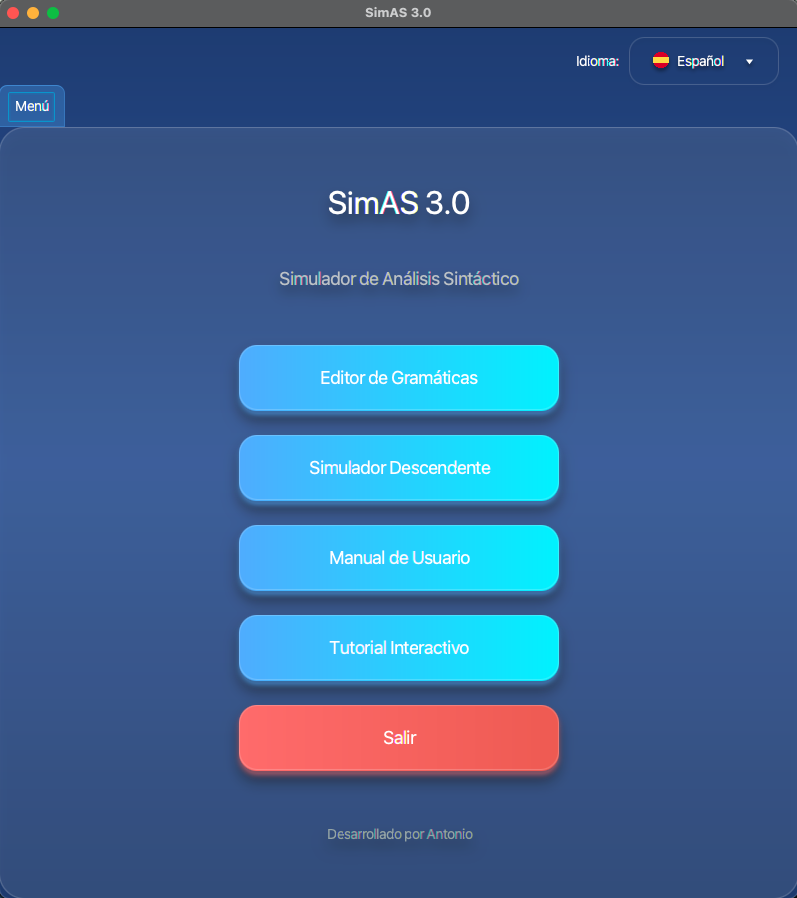
\includegraphics[width=0.8\textwidth]{figuras2/menu.png}
\caption{Menú principal de SimAS.}
\label{fig:d1}
\end{figure}

El menú principal mantiene una estructura consistente y predecible que facilita la navegación, agrupando las funcionalidades relacionadas de manera lógica. Esta organización refleja la arquitectura modular del software, donde cada módulo mantiene su independencia mientras colabora eficientemente con los demás componentes del sistema. 

\section{Barras de herramientas}

Las barras de herramientas constituyen uno de los elementos más importantes de la interfaz de usuario en SimAS 3.0, proporcionando acceso directo e intuitivo a las funciones más utilizadas del sistema. Implementadas como componentes gráficos interactivos, estas barras mejoran significativamente la eficiencia del usuario al reducir la necesidad de navegar por menús complejos.

En el contexto del Editor de gramáticas, la barra de herramientas juega un papel fundamental al ofrecer accesos directos a todas las operaciones relacionadas con la creación, edición y gestión de gramáticas. Esta implementación sigue los principios de diseño de interfaces modernas, priorizando la usabilidad y la accesibilidad.

Una característica técnica destacada de la barra de herramientas es su comportamiento dinámico de habilitación/deshabilitación de controles. Al abrir inicialmente el editor, solo un conjunto limitado de botones permanece activo, específicamente los botones \textbf{Nueva}, \textbf{Abrir} y \textbf{Salir}. Esta estrategia de diseño inteligente previene errores del usuario y guía el flujo de trabajo de manera natural.

En la figura \ref{fig:d2a}, se muestra el estado inicial de la barra de herramientas, donde la mayoría de los controles aparecen deshabilitados para evitar operaciones prematuras.

\needspace{3cm}
\begin{figure}[H]
\centering

\includegraphics[width=0.8\textwidth]{figuras2/editor/barra_herramientas_deshabilita_parcial.png}
\caption{Barra de herramientas con controles parcialmente deshabilitados (estado inicial).}
\label{fig:d2a}
\end{figure}

Una vez que se carga o crea una gramática en el editor, el sistema habilita automáticamente el resto de los controles, permitiendo al usuario acceder a todas las funcionalidades disponibles. Esta transición inteligente refleja la arquitectura de estados del sistema, donde la interfaz se adapta dinámicamente según el contexto de uso.

En la figura \ref{fig:d2}, se muestra la barra de herramientas completamente funcional una vez que se ha cargado una gramática.

\needspace{3cm}
\begin{figure}[H]
\centering
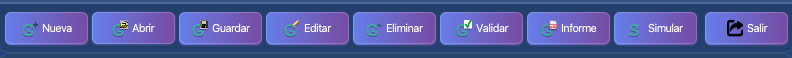
\includegraphics[width=0.8\textwidth]{figuras2/editor/barra_herramientas.png}
\caption{Barra de herramientas completamente funcional.}
\label{fig:d2}
\end{figure}

El diseño de los iconos sigue una convención sistemática que facilita el aprendizaje y la memorización. Se ha procurado que cada botón sea descriptivo y represente fielmente la operación que realiza. Para lograr esto, se ha implementado un sistema de iconos compuesto por una forma base que identifica el objeto involucrado en la operación, complementada con una forma secundaria que representa la acción específica.

Por ejemplo, las operaciones relacionadas con gramáticas están representadas con la letra \textit{G} como forma base, mientras que las operaciones de simulación utilizan la letra \textit{S}. A esta forma base se le superpone gráficamente la acción a realizar, siempre posicionada en la esquina superior derecha del icono. Esta composición visual permite una identificación rápida y precisa de las funcionalidades disponibles.

Esta estrategia de diseño no solo mejora la intuitividad de la interfaz, sino que también optimiza el espacio disponible y reduce la carga cognitiva del usuario. El sistema de habilitación contextual asegura que los usuarios se centren en las tareas apropiadas para cada etapa del proceso, mejorando tanto la eficiencia como la calidad del trabajo realizado.
  

\section{Pestaña \textit{Editor}}

La pestaña del editor representa el módulo principal de creación y gestión de gramáticas en SimAS 3.0. Este componente se abre en una nueva pestaña independiente cuando el usuario selecciona las opciones de crear una nueva gramática o editar una existente desde el menú principal.

El editor proporciona una interfaz completa para el diseño, modificación y validación de gramáticas de contexto libre, facilitando el proceso de preparación de datos para las simulaciones posteriores. Las imágenes mostradas en esta sección corresponden al estado del editor con una gramática activa cargada. Para observar las diferencias con la pestaña del editor vacía, se puede consultar el Manual de Usuario.

La pestaña del editor está compuesta por los siguientes elementos principales:
\begin{enumerate}
 \item \textbf{Barra de herramientas}: proporciona accesos directos a todas las operaciones disponibles.
 \item \textbf{Información de la gramática}: componentes que muestran la información de la gramática activa.
\end{enumerate}

En la figura \ref{fig:d3}, se muestra un ejemplo completo de la pestaña del editor con una gramática activa.

\needspace{8cm}
\begin{figure}[H]
\centering
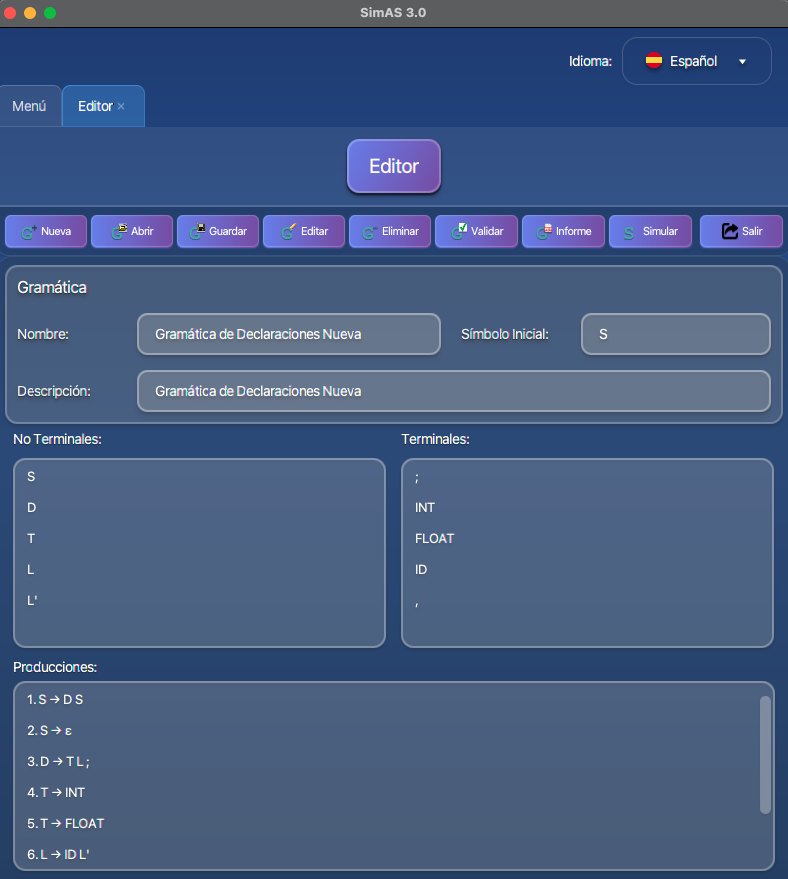
\includegraphics[width=0.9\textwidth]{figuras2/ejemplo_practico/editor.png}
\caption{Pestaña del editor con gramática activa.}
\label{fig:d3}
\end{figure}

La barra de herramientas del editor ya fue detallada en la sección anterior, destacando su sistema inteligente de habilitación/deshabilitación de controles. A continuación se describe la pestaña de edición, que implementa un proceso estructurado de 4 pasos para la creación y modificación de gramáticas.

\subsection{Pestaña \textit{Asistente Editor}}

La pestaña de edición representa la interfaz principal de interacción para la creación y modificación de gramáticas de contexto libre en SimAS 3.0. Esta pestaña se abre inicialmente en el paso 1 del proceso y proporciona un flujo de trabajo guiado que asegura la correcta definición de todos los componentes necesarios para una gramática funcional.

Uno de los aspectos más destacados de esta pestaña es su sistema de navegación inferior, que permite al usuario moverse fluidamente entre los 4 pasos del proceso de edición. Este menú de navegación facilita la revisión y modificación de cualquier paso anterior, proporcionando una experiencia de usuario flexible y no lineal.

El proceso de creación de gramáticas se estructura en 4 pasos secuenciales:

\subsubsection{Paso 1: Nombre y descripción}

El primer paso se centra en la identificación y documentación básica de la gramática. El usuario debe proporcionar:
\begin{itemize}
 \item \textbf{Nombre de la gramática}: un identificador único y descriptivo
 \item \textbf{Descripción}: documentación obligatoria sobre el propósito y características de la gramática
\end{itemize}

En la figura \ref{fig:paso1}, se muestra la interfaz del paso 1 donde se introducen el nombre y la descripción de la gramática.

\needspace{6cm}
\begin{figure}[H]
\centering
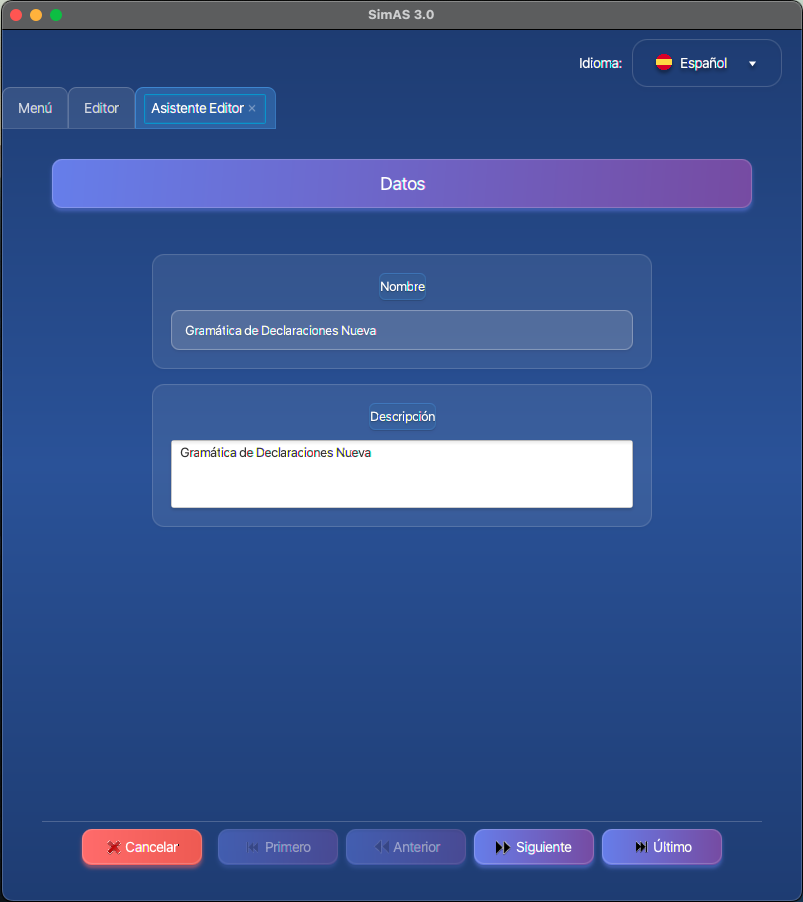
\includegraphics[width=0.8\textwidth]{figuras2/editor/paso1_datos.png}
\caption{Paso 1: Nombre y descripción de la gramática.}
\label{fig:paso1}
\end{figure}

\subsubsection{Paso 2: Símbolos terminales y no terminales}

En este paso se definen los alfabetos fundamentales de la gramática:
\begin{itemize}
 \item \textbf{Símbolos terminales}: el vocabulario básico del lenguaje
 \item \textbf{Símbolos no terminales}: variables que representan construcciones sintácticas
\end{itemize}

La figura \ref{fig:paso2} ilustra la interfaz del paso 2 donde se definen los símbolos terminales y no terminales de la gramática.

\needspace{6cm}
\begin{figure}[H]
\centering
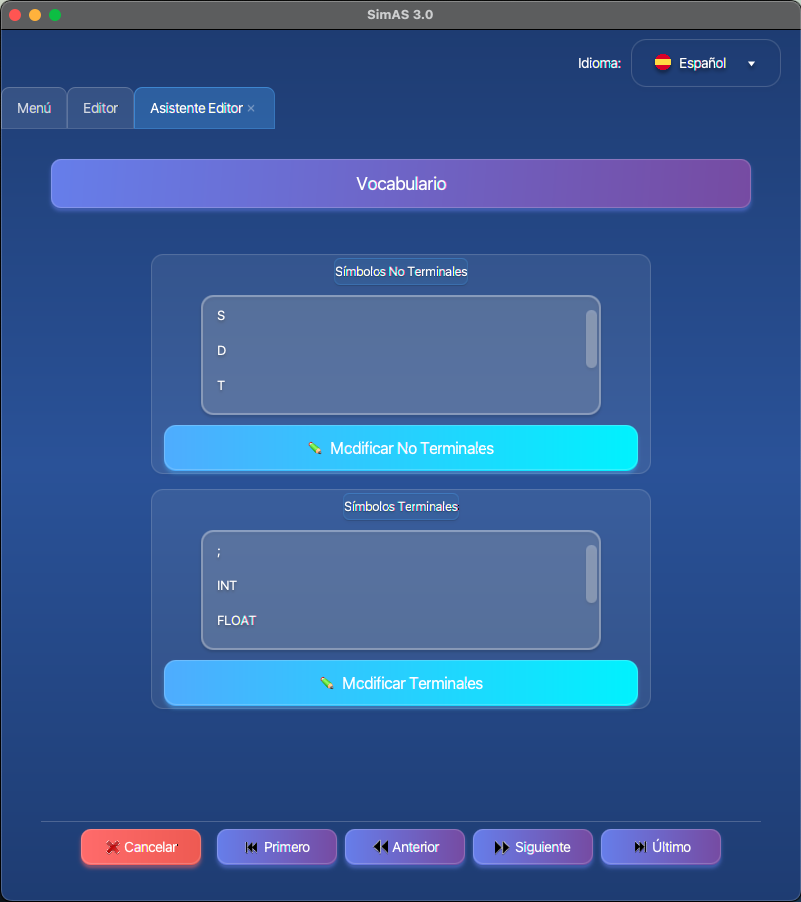
\includegraphics[width=0.8\textwidth]{figuras2/editor/paso2_simbolos.png}
\caption{Paso 2: Definición de símbolos terminales y no terminales.}
\label{fig:paso2}
\end{figure}

\subsubsection{Paso 3: Producciones}

El paso más complejo del proceso, donde se definen las reglas de producción que constituyen el núcleo de la gramática. Cada producción relaciona símbolos no terminales con secuencias de símbolos terminales y no terminales.

En la figura \ref{fig:paso3}, se presenta la interfaz del paso 3 donde se configuran las producciones de la gramática.

\needspace{6cm}
\begin{figure}[H]
\centering
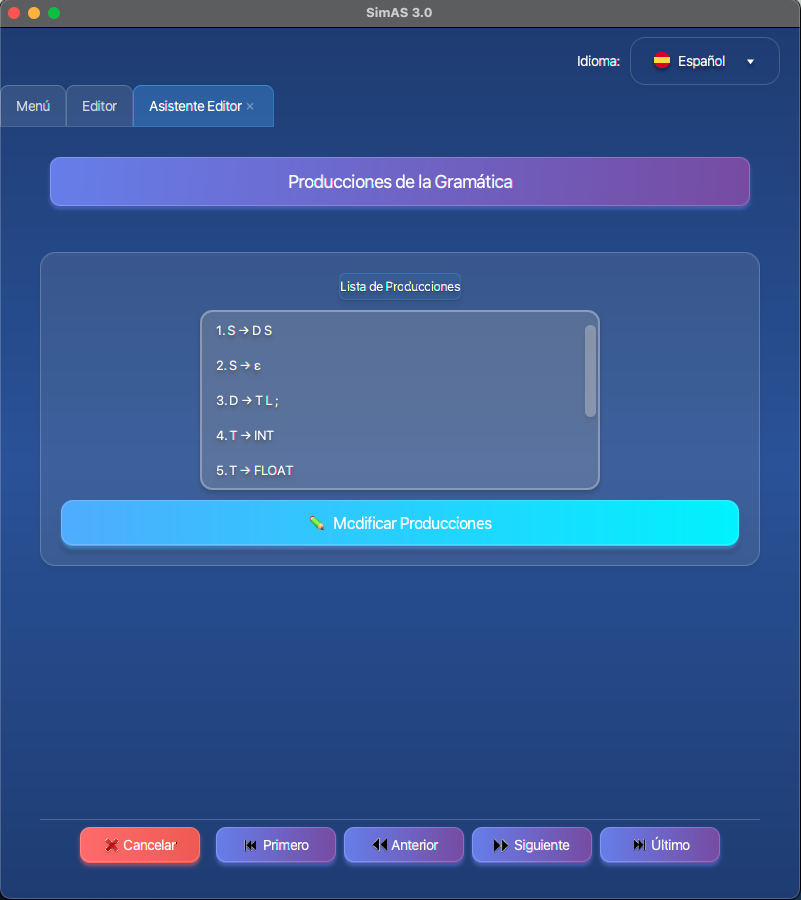
\includegraphics[width=0.8\textwidth]{figuras2/editor/paso3_producciones.png}
\caption{Paso 3: Definición de las producciones de la gramática.}
\label{fig:paso3}
\end{figure}

\subsubsection{Paso 4: Símbolo inicial y validación}

El paso final consolida la definición de la gramática:
\begin{itemize}
 \item \textbf{Símbolo inicial}: selección del símbolo no terminal que inicia el proceso de derivación
 \item \textbf{Validación}: verificación automática de la corrección sintáctica de la gramática
\end{itemize}

La figura \ref{fig:paso4} muestra la interfaz del paso 4 donde se selecciona el símbolo inicial y se realiza la validación final de la gramática.

\needspace{6cm}
\begin{figure}[H]
\centering
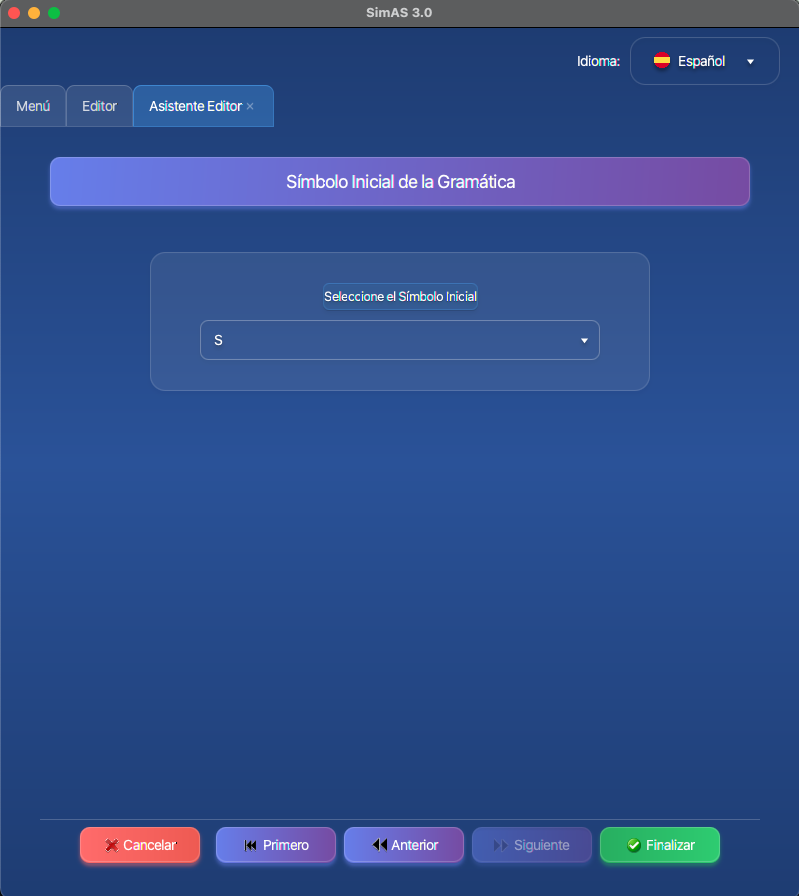
\includegraphics[width=0.8\textwidth]{figuras2/editor/paso4_inicial.png}
\caption{Paso 4: Selección del símbolo inicial y validación de la gramática.}
\label{fig:paso4}
\end{figure}

Esta estructura de 4 pasos proporciona una experiencia de usuario intuitiva y pedagógica, guiando al estudiante a través del proceso de definición de gramáticas de manera sistemática y asegurando que no se omitan componentes esenciales.

\section{Pestaña \textit{Simulador}}

La pestaña del simulador integra tanto el asistente de preparación de gramáticas como la interfaz del simulador propiamente dicho. Esta pestaña se abre cuando el usuario selecciona una gramática preparada y desea proceder con la simulación de análisis sintáctico descendente predictivo.

El asistente integrado en esta pestaña consta de 5 pasos secuenciales que preparan la gramática para la simulación LL(1), seguidos de un sexto paso que corresponde al simulador propiamente dicho.

\subsubsection{Paso 1: Eliminación de recursividad y factorización}

El primer paso del asistente verifica y corrige automáticamente la gramática original para eliminar cualquier recursividad por la izquierda y realizar factorización cuando sea necesario. Este proceso asegura que la gramática cumpla con los requisitos del análisis predictivo LL(1).

En la figura \ref{fig:paso1_sim}, se muestra la interfaz del paso 1 donde se realiza la eliminación de recursividad y factorización de la gramática.

\needspace{6cm}
\begin{figure}[H]
\centering
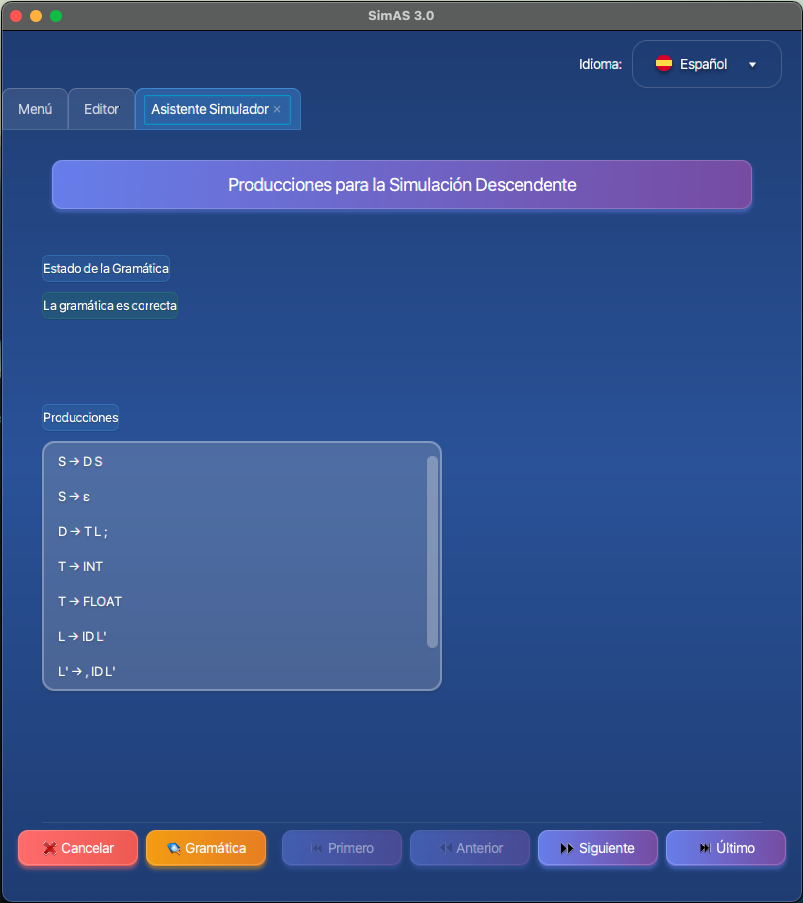
\includegraphics[width=0.8\textwidth]{figuras2/simulador/paso1_recursividad_factorizacion.png}
\caption{Paso 1: Eliminación de recursividad y factorización.}
\label{fig:paso1_sim}
\end{figure}

\subsubsection{Paso 2: Construcción de conjuntos Primero y Siguiente}

En este paso se calculan automáticamente los conjuntos Primero ($\text{First}$) y Siguiente ($\text{Follow}$) para cada símbolo no terminal de la gramática. Estos conjuntos son fundamentales para la construcción de la tabla predictiva y constituyen la base matemática del análisis sintáctico.

La figura \ref{fig:paso2_sim} ilustra la interfaz del paso 2 donde se muestran los conjuntos Primero y Siguiente calculados para la gramática.

\needspace{6cm}
\begin{figure}[H]
\centering
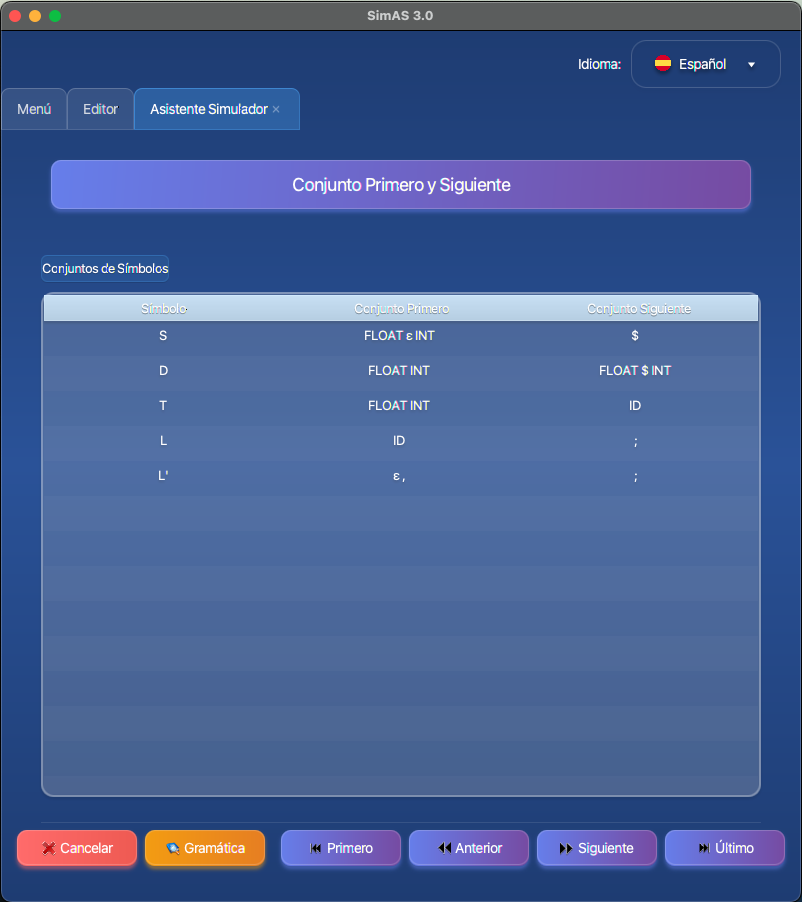
\includegraphics[width=0.8\textwidth]{figuras2/simulador/paso2_conjuntos.png}
\caption{Paso 2: Construcción de conjuntos Primero y Siguiente.}
\label{fig:paso2_sim}
\end{figure}

\subsubsection{Paso 3: Construcción de la tabla predictiva}

El asistente construye la tabla predictiva LL(1) utilizando los conjuntos calculados en el paso anterior. Esta tabla determina, para cada combinación de símbolo no terminal y símbolo terminal, cuál es la producción que debe aplicarse durante el análisis.

En la figura \ref{fig:paso3_sim}, se presenta la interfaz del paso 3 donde se construye la tabla predictiva LL(1).

\needspace{6cm}
\begin{figure}[H]
\centering
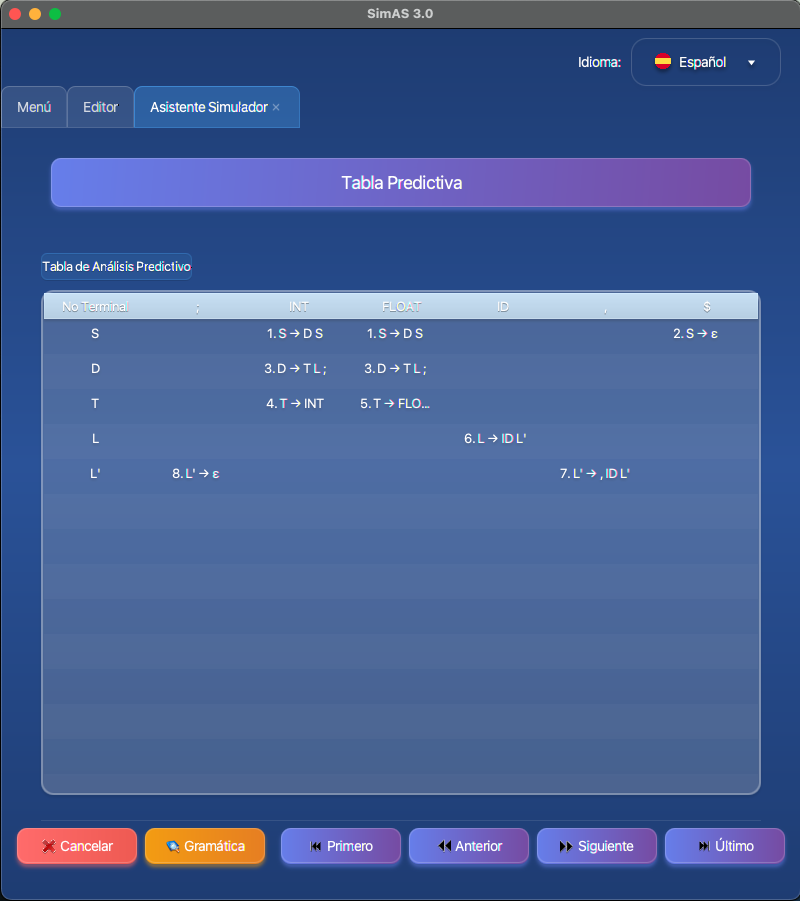
\includegraphics[width=0.8\textwidth]{figuras2/simulador/paso3_tablaPredictiva.png}
\caption{Paso 3: Construcción de la tabla predictiva.}
\label{fig:paso3_sim}
\end{figure}

\subsubsection{Paso 4: Definición de funciones de error}

El sistema predefine automáticamente algunas funciones de error básicas, pero permite al usuario personalizar y definir funciones de error adicionales según sus necesidades específicas. Las funciones de error son cruciales para el manejo adecuado de situaciones de error durante el análisis sintáctico.

La figura \ref{fig:paso4_sim} muestra la interfaz del paso 4 donde se definen y configuran las funciones de error para la simulación.

\needspace{6cm}
\begin{figure}[H]
\centering
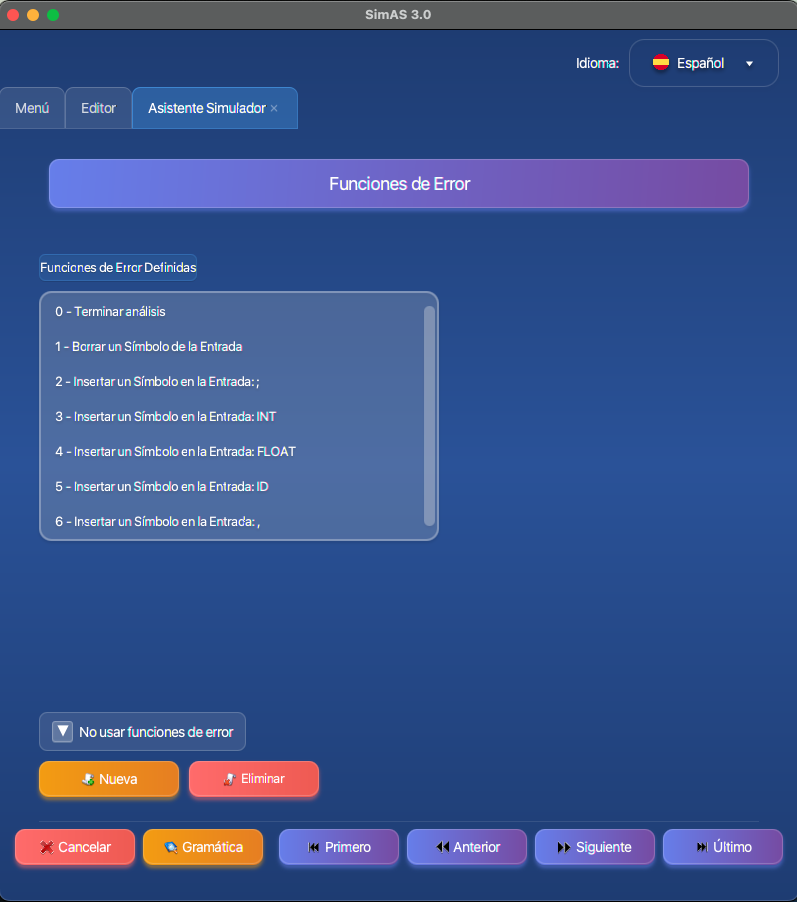
\includegraphics[width=0.8\textwidth]{figuras2/simulador/paso4_funcionesError.png}
\caption{Paso 4: Definición de funciones de error.}
\label{fig:paso4_sim}
\end{figure}

\subsubsection{Paso 5: Construcción interactiva de la tabla predictiva final}

En el último paso del asistente, el usuario puede revisar y modificar interactivamente la tabla predictiva, añadiendo las funciones de error definidas en el paso anterior. Esta construcción interactiva permite al usuario tener un control total sobre el comportamiento del analizador.

En la figura \ref{fig:paso5_sim}, se muestra la interfaz del paso 5 donde el usuario puede construir interactivamente la tabla predictiva final incorporando las funciones de error.

\needspace{6cm}
\begin{figure}[H]
\centering
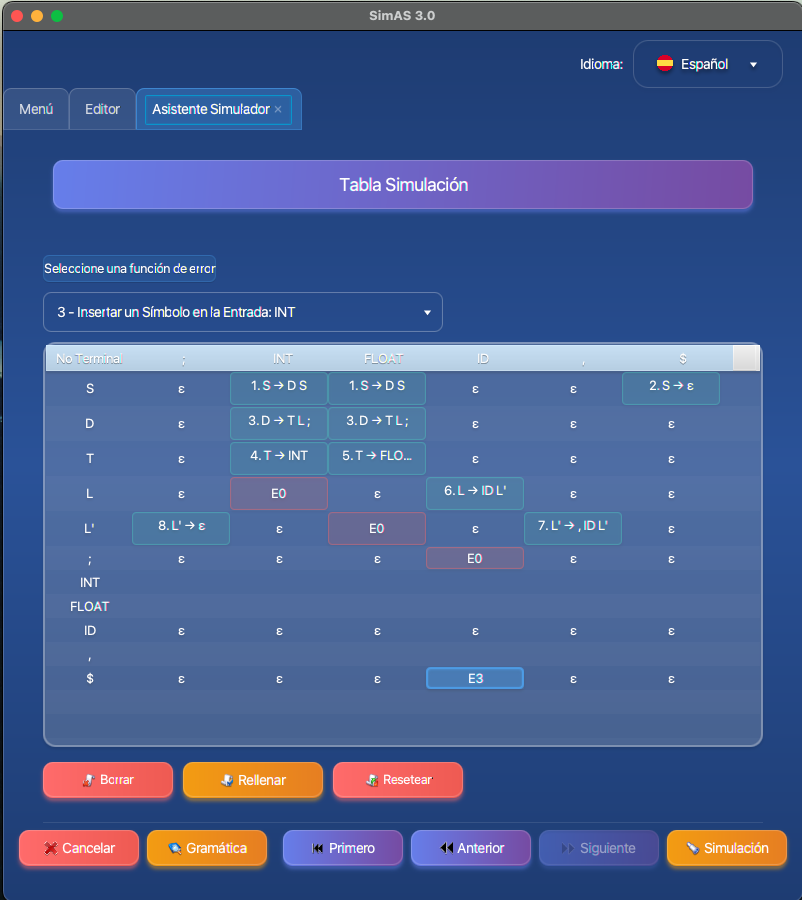
\includegraphics[width=0.8\textwidth]{figuras2/simulador/paso5_tablaPredictivaCompleta.png}
\caption{Paso 5: Construcción interactiva de la tabla predictiva final.}
\label{fig:paso5_sim}
\end{figure}

\subsubsection{Paso 6: Simulador (Resumen y ejecución)}

Una vez completados los 5 pasos del asistente, se accede al simulador propiamente dicho, que actúa como resumen de todo el proceso preparatorio. El simulador contiene:

\begin{itemize}
 \item \textbf{Producciones modificadas}: las reglas de producción preparadas para simulación LL(1)
 \item \textbf{Funciones de error definidas}: el conjunto completo de funciones de error configuradas
 \item \textbf{Tabla predictiva completa}: la tabla final que se utilizará en la simulación
\end{itemize}

En la figura \ref{fig:simulador}, se muestra la interfaz del simulador en funcionamiento, donde se integran las producciones modificadas, funciones de error y tabla predictiva completa preparadas para la simulación.

\needspace{8cm}
\begin{figure}[H]
\centering
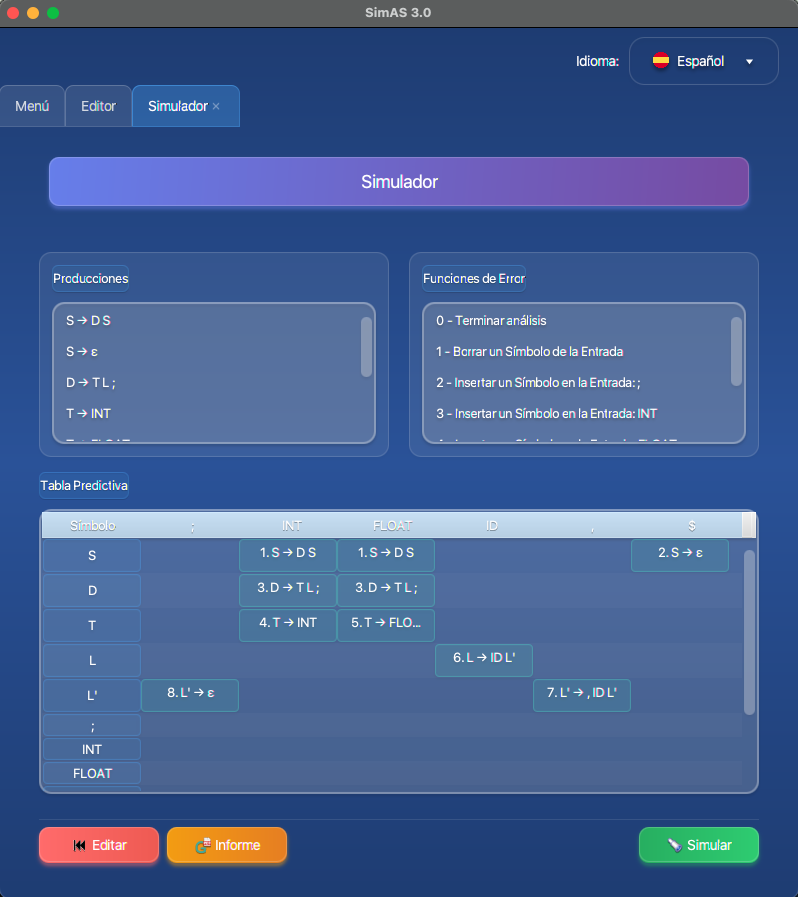
\includegraphics[width=0.8\textwidth]{figuras2/simulador/simulador.png}
\caption{Simulador con producciones modificadas y tabla predictiva completa.}
\label{fig:simulador}
\end{figure}

El simulador proporciona capacidades avanzadas de documentación y navegación:

\begin{itemize}
 \item \textbf{Generación de informes}: capacidad de generar informes detallados con toda la información necesaria para la simulación, incluyendo producciones modificadas, funciones de error y tabla predictiva completa
 \item \textbf{Llave de navegación}: actúa como punto de acceso principal para abrir las pestañas de simulación individual, permitiendo al usuario ejecutar análisis sintácticos paso a paso
\end{itemize}

Esta integración del asistente y el simulador en una sola pestaña proporciona una experiencia de usuario coherente y eficiente, permitiendo tanto la preparación automática de la gramática como la ejecución interactiva de simulaciones.

\subsection{Pestaña \textit{Gramática Original}}

La pestaña de Gramática Original representa una innovadora funcionalidad pedagógica introducida en SimAS 3.0, que no estaba disponible en versiones anteriores del software. Esta característica se activa mediante el botón \string"Gramática\string" ubicado en el menú inferior de navegación, el cual permanece visible y accesible durante todos los pasos del asistente de simulador.

Esta funcionalidad permite al usuario mantener una referencia visual constante de la gramática original mientras observa cómo el sistema la transforma y prepara para el análisis LL(1). A medida que se generan los diferentes conjuntos, tablas y funciones de error a través de los 5 pasos del asistente, el usuario puede consultar en cualquier momento la gramática original para realizar comparaciones pedagógicas y comprender mejor las transformaciones aplicadas.

\subsubsection{Propósito pedagógico y técnico}

La pestaña cumple un doble propósito tanto educativo como técnico:

\begin{itemize}
 \item \textbf{Propósito educativo}: permite al estudiante comparar visualmente cómo la gramática original se transforma durante el proceso de eliminación de recursividad por la izquierda y factorización, facilitando la comprensión de estos conceptos fundamentales del análisis sintáctico.

 \item \textbf{Propósito técnico}: ofrece una referencia constante que ayuda al usuario a verificar que las transformaciones aplicadas mantienen la equivalencia semántica con la gramática original, asegurando la corrección del proceso de preparación.
\end{itemize}

\subsubsection{Disponibilidad y accesibilidad}

A diferencia de otras funcionalidades que se activan solo en ciertos pasos, el botón de acceso a la gramática original permanece disponible durante toda la sesión del asistente, permitiendo al usuario:

\begin{itemize}
 \item Consultar la gramática original en cualquier momento del proceso
 \item Realizar comparaciones entre la gramática original y las versiones transformadas
 \item Verificar visualmente las modificaciones aplicadas en cada paso
 \item Mantener una referencia contextual durante todo el proceso de preparación
\end{itemize}

La pestaña se presenta como un panel simple y limpio que muestra la gramática original en el mismo formato visual utilizado para las gramáticas modificadas, facilitando las comparaciones directas. En la figura \ref{fig:gramatica_original}, se muestra un ejemplo de esta interfaz.

\needspace{8cm}
\begin{figure}[H]
\centering
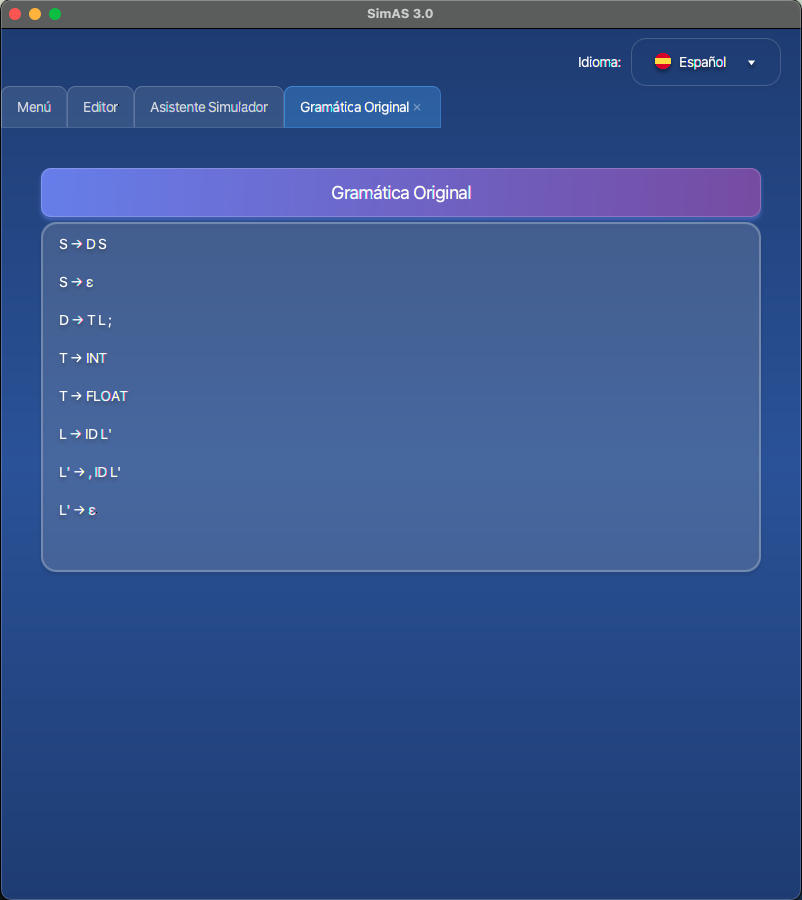
\includegraphics[width=0.8\textwidth]{figuras2/simulador/gramatica_original.png}
\caption{Pestaña de visualización de la gramática original.}
\label{fig:gramatica_original}
\end{figure}

Esta funcionalidad representa un avance significativo en la interfaz pedagógica de SimAS, proporcionando una herramienta visual que facilita el aprendizaje de los conceptos de transformación de gramáticas y su importancia en el análisis sintáctico descendente predictivo.

\section{Pestaña \textit{Simulación}}

La pestaña de simulación se encarga de ejecutar las simulaciones de una cadena de entrada. En la figura \ref{fig:d7}, se muestra un ejemplo de esta pestaña.

La pestaña está compuesta de los siguientes elementos:
\begin{enumerate}
  \item \textbf{Tipo de análisis}: muestra el tipo de simulación que se va a llevar a cabo, \textit{descendente} o \textit{ascendente}. En el caso de ser la simulación del análisis ascendente, también se detalla el tipo: \textit{SLR}, \textit{LR-canónico} o \textit{LALR}.
 \item \textbf{Cadena de entrada}: permite introducir los símbolos terminales que forman parte de la cadena de entrada que se va a simular.
 \item \textbf{Botones de Avance y Retroceso}: la simulación se podrá realizar paso a paso o de forma completa, pudiendo avanzar y retroceder en cada paso.
 \item \textbf{Tabla de análisis}: representa la tabla de resultados del análisis.
 \item \textbf{Generar Árbol Sintáctico}: permite abrir una pestaña en la que se genere el árbol sintáctico correspondiente.
 \item \textbf{Generar Derivación}: permite abrir una pestaña en la que se genere la derivación de la simulación correspondiente.
 \item \textbf{Informe de la Simulación}: permite al usuario generar un informe en pdf de la simulación.
\end{enumerate}

\begin{figure}[htp]
\centering
	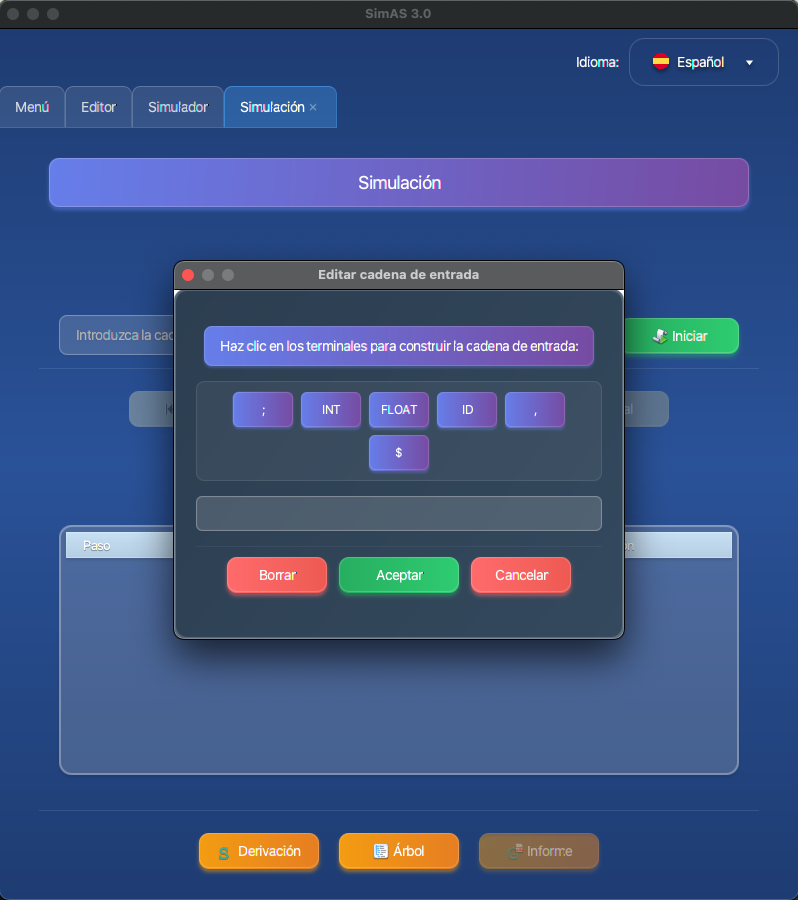
\includegraphics[width=0.8\textwidth]{figuras2/simulador/simulacion_cadenaEntrada.png}
	\caption{Pestaña de simulación.}
	\label{fig:d7}
\end{figure}

\section{Pestaña \textit{Árbol Sintáctico}}

El árbol sintáctico se podrá ver en una pestaña la cual se irá repintando a medida que se continue con la simulación (Figura \ref{fig:da22}).

\begin{figure}[htp]
\centering
	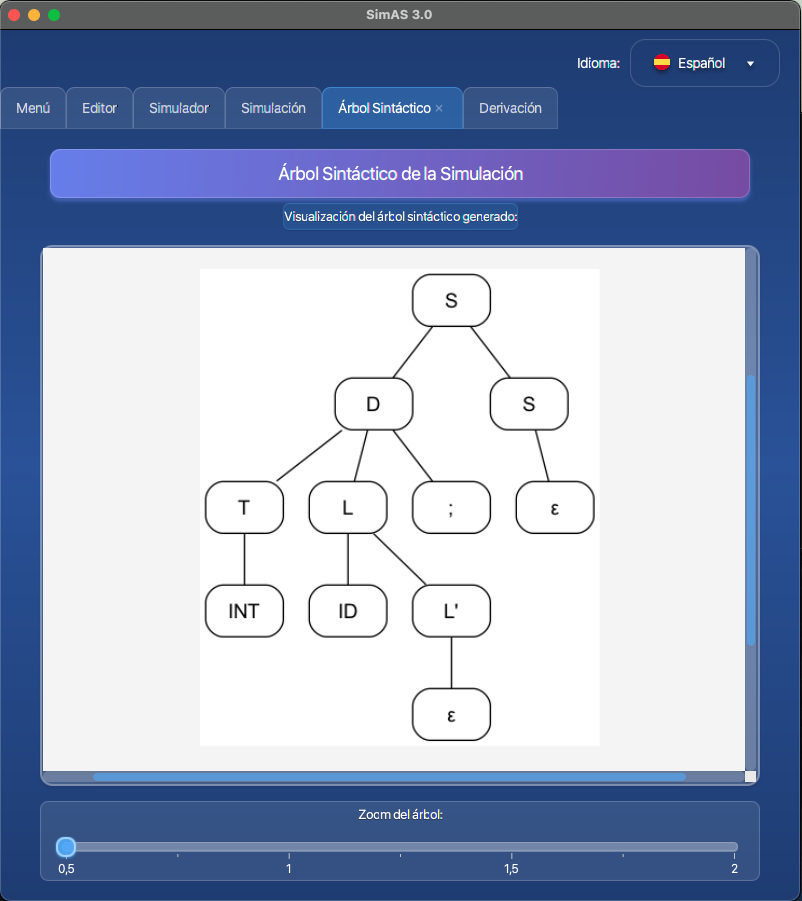
\includegraphics[width=0.8\textwidth]{figuras2/simulador/simulacion_arbol.png}
	\caption{Pestaña de simulación.}
	\label{fig:da22}
\end{figure}

\section{Pestaña \textit{Derivación}}

Además del árbol, es posible generar la derivación de la simulación actual en una pestaña adicional tal y como se muestra en la imagen \ref{fig:da24}:

\begin{figure}[htp]
\centering
	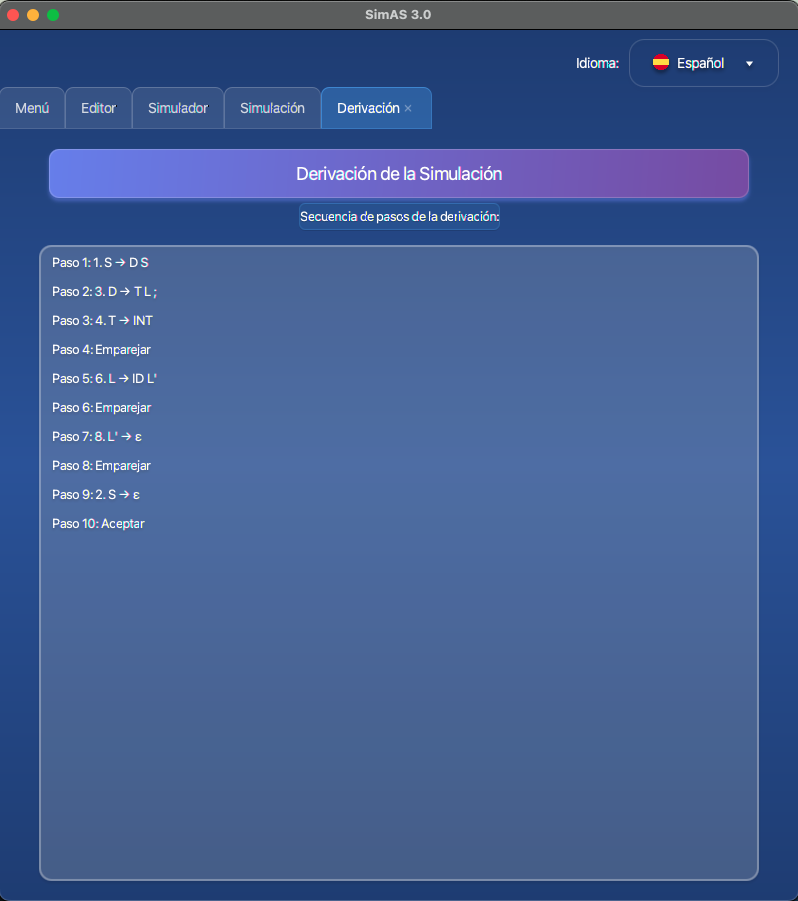
\includegraphics[width=0.8\textwidth]{figuras2/simulador/simulacion_derivacion.png}
	\caption{Pestaña de simulación.}
	\label{fig:da24}
\end{figure}